\chapter{Fundamentação Teórica}

\section{Aprendizado de máquina}

Aprendizado de máquina, ou \textit{Machine Learning}, é uma área da
computação que emergiu de estudos relacionados ao reconhecimento de
padrões e inteligência artificial. Nesta área é contemplado o estudo e
implementação de algoritmos que conseguem aprender e fazer previsões
baseadas em dados. Esses algoritmos funcionam através da construção de
um modelo preditivo que tem como entrada um conjunto de treinamento
com dados de observações quaisquer. Desse modo as previsões são feitas
orientadas aos dados e não a partir de instruções estáticas de um
programa.

\section{Redes Neurais}

Diante das ferramentas disponíveis que tratam de aprendizado de
máquina, uma delas é a rede neural artificial.

Redes neurais artificiais são conjuntos de modelos inspirados por
redes neurais biológicas, usados para aproximar funções que dependem
de um número muito grande de entradas. De acordo com Mackay\cite{Mackay},
redes neurais geralmente são especificadas utilizando 3 coisas:

\begin{itemize}

\item {\bf Arquitetura:} Especifica quais variáveis estão envolvidas
  na rede e quais as relações topológicas. Por exemplo, as variáveis
  envolvidas em uma rede neural podem ser os pesos das conexões entre
  os neurônios.

\item {\bf Regra de atividade:} A maioria dos modelos de rede neural
  tem uma dinâmica de atividade com escala de tempo curta. São regras
  locais que definem como as ``atividades'' de neurônios mudam em
  resposta aos outros. Geralmente a regra de atividade depende dos
  parâmetros da rede.

\item {\bf Regra de aprendizado:} Especifica o modo com que os pesos
  da rede neural muda conforme o tempo. O aprendizado normalmente toma
  uma escala de tempo maior do que a escala referente a dinâmica de
  atividade. Normalmente a regra de aprendizado dependerá das
  ``atividades'' dos neurônios. Também pode depender dos valores
  que são objetivos definidos pelo usuário e valores iniciais dos
  pesos.

\end{itemize}

Tomando imagens como exemplo, uma rede neural para reconhecimento de
texto pode ter como entrada o conjunto de pixels\footnote{pixel é o
  menor ponto que forma uma imagem digital, sendo que o conjunto de
  milhares de pixels formam a imagem inteira. Cada Pixel é composto
  por um conjunto de 3 pontos: verde, vermelho e azul.} da
imagem. Depois de serem atribuídos os pesos para cada item da entrada,
os próximos neurônios serão ativados mediante a função de atividade
pré-definida. Os pesos são recalculados através da regra de
aprendizado e todo processo é repetido até uma condição determinada
pelo usuário.

\section{Regressão logística multinomial}

Regressão logística multinomial é um método de classificação que
consiste em um modelo que é usado para prever probabilidades de
variáveis associadas a uma determinada classe, baseado em um conjunto
de variáveis independentes. Para construir este modelo, esta seção
descreve as tarefas e cálculos principais.

\subsection{Classificação supervisionada}

Classificação é uma tarefa central para o aprendizado de máquina, e
consiste em receber uma entrada, como a imagem da letra ``A'' por
exemplo, e dar um rótulo que diz que essa imagem é da classe
``A''. Geralmente temos muitos exemplos da entidade que queremos
classificar. Esses exemplos já mapeados com seu respectivo rótulo, são
chamados de conjunto de treinamento. Após o treinamento o objetivo é
receber um exemplo completamente novo e descobrir em qual classe esse
exemplo se encaixa.

É dito que esse aprendizado é supervisionado pois cada exemplo
recebeu um rótulo durante o treinamento. Já o aprendizado não
supervisionado não conhece os rótulos de cada exemplo, mas tenta
agrupar os exemplos que possuem semelhança baseado em propriedades
úteis encontradas ao longo do treinamento.

\subsection{Classificador Logístico}

Um classificador logístico, ou linear, recebe como entrada os pixels
de uma imagem por exemplo, e aplica uma função linear a eles para
gerar suas predições. Uma função linear é apenas uma grande
multiplicação de matriz. Recebe todas as entradas como um grande vetor
que será chamado de ``X'', e multiplica os valores desse vetor com uma
matriz para gerar as predições, cada predição é como uma pontuação,
que possui o valor que indica o quanto as entradas se encaixam em uma
classe de saída.

\begin{equation}
   WX + b = Y
\end{equation}

``X'' é como chamaremos o vetor das entradas, ``W'' serão pesos e
o termo tendencioso (\textit{bias}) será representado por ``b''. ``Y''
corresponde ao vetor de pontuação para cada classe. Os pesos da
matriz e o \textit{bias} é onde age o aprendizado de máquina, ou seja,
é necessário tentar encontrar valores para os pesos e para o
\textit{bias} que terão uma boa performance em fazer predições para as
entradas.

\subsection{Inicialização de pesos Xavier}

Uma tarefa crucial para o sucesso na construção de redes neurais é a
inicialização da matriz de pesos. Geralmente os pesos são
inicializados de maneira aleatória. No caso do trabalho proposto,
os valores serão inicializados de forma aleatória seguindo uma regra
de distribuição, utilizando a inicialização de Xavier\cite{Glorot}.

Se os pesos forem inicializados com um valor muito baixo, é capaz que
as ativações da rede neural diminuam ao passar por cada camada. Já com
uma inicialização de valores muito altos para o peso, as ativações
podem acabar crescendo demais ao longo das camadas. A inicialização de
Xavier garante que os pesos serão inicializados na ``medida certa'',
mantendo as ativações em uma variação razoável de valores mediante
várias camadas da rede neural. A distribuição segue a seguinte
fórmula:

\begin{equation}
  Var(W) = \frac{2}{n_{in}+n_{out}}
\end{equation}

Onde $W$ é a distribuição da inicialização para o peso em questão,
$n_{in}$ é o número de neurônios de entrada, e $n_{out}$ é o número de
neurônios de saída.

\subsection{Função Softmax}

Como cada imagem pode ter um e somente um rótulo possível, é necessário
transformar essas pontuações em probabilidades. Queremos que a
probabilidade de ser a classe correta seja muito perto de {\bf 1.0} e
a probabilidade para todas as outras classes fique perto de {\bf
  0.0}.
Para tornar essas pontuações em probabilidades utilizamos uma função
chamada {\bf \emph{Softmax}}. Denotada na equação por ``S''.

\begin{equation}
   S(y_i) = \displaystyle\frac{e^{y_i}}{\displaystyle\sum_{j} e^{y_j}}
\end{equation}

O mais importante dessa fórmula é que pode receber qualquer tipo de
pontuação gerado por predições e transformá-la em probabilidades
adequadas. Os valores dessas probabilidades serão altos quando a
pontuação da classe for alta e baixos quando a pontuação da classe for
baixa. A soma das probabilidades fica igual a 1.

Ao final do processo de aplicação da função linear e da função
Softmax temos um vetor de tamanho igual ao número de classes possíveis
e em cada posição do vetor temos a probabilidade para a classe
referente a essa específica posição do vetor.

\subsection{One-Hot Encoding}

Para facilitar o treinamento é preciso representar de forma matemática
os rótulos de cada exemplo que iremos alimentar a rede neural. Cada
rótulo será representado por um vetor de tamanho igual ao número de
classes possíveis, assim como o vetor de probabilidades. No caso dos
rótulos, será atribuído o valor de {\bf 1.0} para a posição referente
a classe correta daquele exemplo e {\bf 0.0} para todas as outras
posições. Essa tarefa é bem simples e geralmente chamada de
\textit{One-Hot Encoding}. Com isso é possível medir a eficiência do
treinamento apenas comparando 2 vetores.

\subsection{Cross Entropy}

O jeito mais comum em redes neurais de profundidade para medir a
distância entre o vetor de probabilidades e o vetor correspondente ao
rótulo se chama {\bf \emph{cross entropy}}.

\begin{equation}
   D(S,L) = - \displaystyle\sum_{i}L_i  {\log (S_i)}
\end{equation}

Na equação o \textit{cross entropy} é representado por ``D'' que é a
distância. ``S'' é o vetor de probabilidades vindo da função
\textit{Softmax} e ``L'' é o vetor referente ao rótulo do exemplo em
questão.

\subsection{Treinamento}

Com todas as tarefas e cálculos disponíveis, resta descobrir os
valores dos pesos e \textit{biases} mais adequados ao modelo de
regressão.

\subsubsection{Perda}

Para cada valor aleatório de peso e \textit{bias}, é possível medir a
distância média para todas as entradas de todo o conjunto de
treinamento e todos rótulos que estão disponíveis. Esse valor é
chamado de {\bf perda} do treinamento. Esta perda, que é a média de
\textit{cross entropy} de todo treinamento, é uma função grande e
custosa.

\begin{equation}
  L = \displaystyle\frac{1}{N}\displaystyle\sum_iD(S(WX_i + b), L_i)
\end{equation}

Cada exemplo no conjunto de treinamento é multiplicado por uma grande
matriz ``W''. Depois é tudo adicionado em um grande somatório.

O objetivo é que as distâncias sejam minimizadas, o que significa que a
classificação está indo bem para todos os exemplos dos dados de
treinamento. Portanto queremos que a perda seja pequena. A
perda nada mais é que uma função em relação aos pesos e
\textit{biases}. Assim é necessário tentar minimizar essa função,
tornando um problema de aprendizado de máquina em um problema de
otimização numérica.

\subsection{Overfitting}

Segundo Goodfellow\cite{Goodfellow-et-al-2016-Book},no aprendizado de
máquina há dois fatores que são desafios centrais para os
pesquisadores: \textit{underfitting} e
\textit{overfitting}. \textit{Underfitting} acontece quando o modelo
não está apto para obter um valor de perda suficientemente baixo com o
conjunto de dados de treinamento. Isso varia de acordo com o problema
que se está querendo resolver.

Já o \textit{overfitting} ocorre quando a diferença é muito grande
entre o valor de perda para o conjunto de treinamento e o valor de
perda para o conjunto de teste. É possível controlar se um modelo fica
mais propenso ao \textit{overfit} ou ao \textit{underfit} alterando
sua {\bf capacidade}. Informalmente, a capacidade de um modelo é sua
habilidade de se encaixar em uma grande variedade de funções. Modelos
com baixa capacidade terão mais trabalho para se encaixar em um
conjunto de dados. Enquanto modelos com alta capacidade podem se
encaixar muito bem e acabar memorizando propriedades do conjunto de
treinamento que não servem para o conjunto de teste.

\subsection{Método do Gradiente}

O jeito mais simples de otimização numérica é utilizando método do
gradiente (ou \textit{Gradient Descent} em inglês).

\begin{equation}
  w \leftarrow w - \alpha \Delta_w L
\end{equation}
\begin{equation}
  b \leftarrow b - \alpha \Delta_b L
\end{equation}

Este método calcula a derivada da função de perda em relação a cada
peso(w) e cada \textit{bias}(b), assim computando um novo valor para
essas variáveis e indo na direção oposta à derivada.

Para o treinamento funcionar esse processo será executado dezenas ou
centenas de vezes até encontrar os valores ideais de pesos e
\textit{biases}.

\begin{figure}[H]
\centering
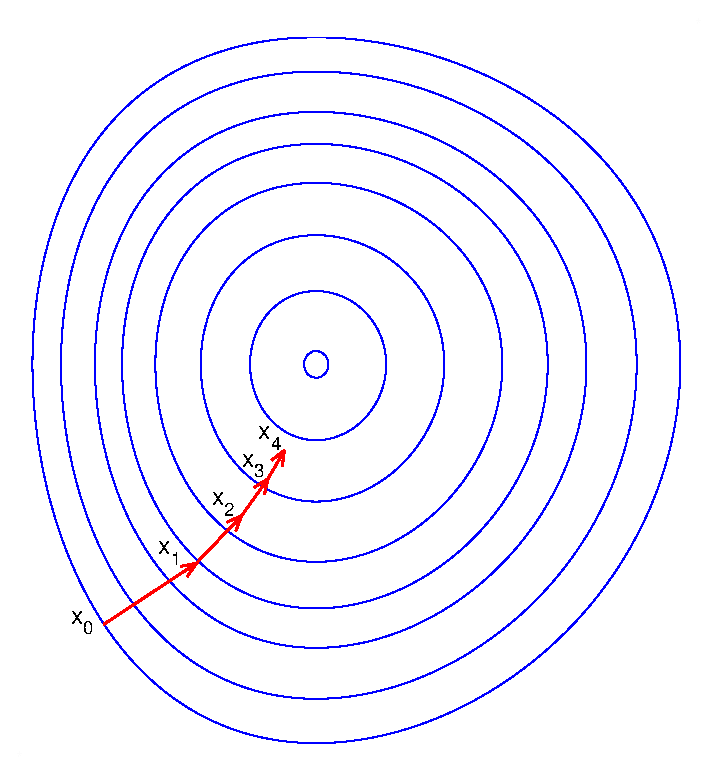
\includegraphics[scale=0.6]{imagens/Gradient_descent.eps}
\caption{Os círculos na imagem representam a função de perda quando há
  apenas 2 parâmetros de peso como exemplo, a função será maior em
  algumas áreas e menor em outras. Tentaremos encontrar os pesos que
  fazem com que a perda seja reduzida. Portanto o método do Gradiente
  irá calcular a derivada da perda em relação aos parâmetros de peso e
  dar um passo na direção oposta ($x_0,x_1,...,x_n$), que significa
  calcular novos pesos para minimizar a perda.}
\label{fig:gradient_descent}
\end{figure}

\section{Aprendizado em profundidade}

O aprendizado em profundidade permite que modelos computacionais
compostos por múltiplas camadas de processamento possam aprender
representações de dados com múltiplos níveis de abstração\cite{LeCun}.
Essa técnica de aprendizado começa a ficar mais famosa depois de 2
adventos específicos da computação: a geração de enormes volumes de
dados e a utilização de GPUs para propósitos gerais (GPGPU).

A solução de \textit{Deep learning} permite que computadores aprendam
a partir de experiências e entendam o mundo em termos de uma
hierarquia de conceitos, com cada conceito definido em termos da sua
relação com conceitos mais simples. Juntando conhecimento de
experiência, essa abordagem evita a necessidade de ter operadores
humanos especificando formalmente todo o conhecimento que o computador
precisa. A hierarquia de conceitos permite que o computador aprenda
conceitos complexos construindo-os à partir de conceitos mais
simples. Desenhando um gráfico que mostra como esses conceitos são
construídos em cima de outros, o gráfico fica profundo, com muitas
camadas. Por esta razão, essa abordagem para IA é chamada de
Aprendizado em profundidade\cite{Goodfellow-et-al-2016-Book}.

\subsection{Otimização com SGD}

O algoritmo SGD (do inglês, \textit{Stochastic Gradient Descent}) é
uma peça chave de \textit{Deep learning}. Praticamente todo o
aprendizado em profundidade é alimentado por esse algoritmo muito
importante. O problema do método do Gradiente visto anteriormente, é
que o mesmo se torna muito difícil de escalar. Para cada vez que é
calculada a perda do modelo, um computador pode levar em torno de 3
vezes esse tempo para calcular o gradiente.

Como foi dito anteriormente, um ponto crucial do aprendizado em
profundidade é a utilização de uma grande quantidade de dados. Visto o
tempo e a ineficiência do método do Gradiente, no algoritmo SGD é
feita uma adaptação para realizar o treinamento sobre um conjunto de
dados maior. Ao invés de calcular a perda, será calculada uma
estimativa dessa perda. Esta estimativa será feita baseada na perda
calculada para uma pequena parte do conjunto de dados do
treinamento. Essa pequena fração terá entre 1 e 1000 exemplos dos
dados e precisa ser escolhida aleatoriamente do conjunto de
treinamento. Utilizando este método, a perda pode aumentar em alguns
momentos, mas isto será compensado pois será possível executar esse
processo muito mais vezes do que com o método do Gradiente
comum. Ao longo do tempo, executar esses procedimentos por milhares ou
milhões de vezes é muito mais eficiente do que utilizar somente o
método do Gradiente.

\subsection{Momentum}

Em cada iteração do processo de treinamento, será tomado um passo bem
pequeno em uma direção aleatória que seria a mais indicada para
diminuir a perda. Mas ao agregar todos esses passos chegamos na função
com perda mínima. É possível tomar vantagem do conhecimento acumulado
de passos anteriores para saber qual direção tomar. Um jeito barato de
fazer isto é manter uma média móvel\footnote{Média móvel é um cálculo
  que analisa pontos de dados criando séries de médias de diferentes
  subconjuntos de um conjunto completo de dados} de todos os
gradientes, e usar essa média móvel ao invés da direção do atual
conjunto de dados. Essa técnica é chamada de \textit{momentum} e
geralmente leva a uma convergência melhor.

\subsection{Declínio da taxa de aprendizado}

Como foi dito anteriormente, em cada etapa do processo de treinamento
é tomado um pequeno passo em direção a minimização da perda. A {\bf
  taxa de aprendizado} é o parâmetro que diz o quão pequeno é esse
passo. Existe uma área inteira de pesquisa sobre essa taxa, e os
melhores resultados indicam que é mais apropriado decair a taxa de
aprendizado ao longo do treinamento. Neste trabalho iremos aplicar
um declínio exponencial à taxa de aprendizado.\cite{Zeiler}

\subsection{ReLU}

Modelos lineares são simples e estáveis numéricamente mas podem se
tornar ineficientes ao longo do tempo. Portanto para adicionar mais
camadas ao modelo, será necessário introduzir alguns cálculos
não lineares entre camadas. Em arquiteturas de profundidade, as
funções de ativação dos neurônios se chamam ReLUs, e são capazes de
introduzir cálculos não lineares aos modelos que possuem mais de uma
camada. Essas são as funções não lineares mais simples que
existem, elas são lineares ($y=x$) se {\bf x} é maior que {\bf 0},
senão ficam iguais a {\bf 0} ($y=0$). Isso simplifica o uso de
\textit{backpropagation} e evita problemas de saturação, fazendo o
aprendizado ficar muito mais rápido.

\begin{figure}[H]
\centering
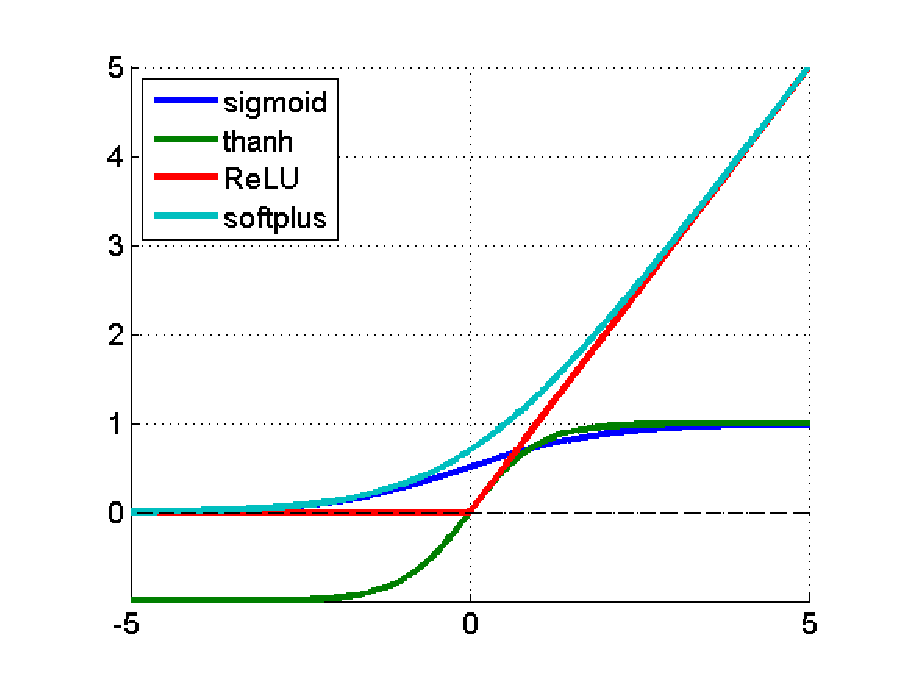
\includegraphics[scale=0.6]{imagens/activation_funcs.eps}
\caption{Comparação de funções de ativação.}
\label{fig:activation_funcs}
\end{figure}

\subsubsection{Camada oculta}

Como as unidades ReLU não precisam de parâmetros e não são observáveis
fora da rede, a introdução dessas unidades entre camadas do modelo é
chamada de camada oculta e pode possuir quantas unidades for
necessário para uma melhor performance.

\subsection{Backpropagation}

\textit{Backpropagation} é um método que faz o cálculo de derivadas de
funções complexas eficientemente, contanto que estas funções sejam
feitas de funções menores que possuem derivadas simples.

\subsubsection{Regra da cadeia}

Um motivo de construir uma rede juntando operações simples é que torna
a matemática muito mais simples. Com a regra da cadeia é possível
concluir que para calcular a derivada de funções compostas, precisamos
apenas calcular o produto das derivadas dos componentes.

Utilizando o método da cadeia, a maioria dos frameworks de aprendizado
de máquina implementa o conceito de \textit{backpropagation}
automaticamente para o usuário. Assim é possível reutilizar dados
pré-calculados e potencializar a eficiência do processo de
treinamento.

\subsection{Regularização}

Regularizar significa aplicar restrições artificiais em sua rede que
fazem com que o número de parâmetros livres reduza e isso não aumente
a dificulade para otimizar. Essa é uma das formas de previnir o
\textit{overfitting} no modelo pois adicionamos um fator externo
que torna a rede mais flexível.

\subsubsection{Regularização com $L_2$}

A ideia é adicionar um termo a mais à perda, o que dá uma penalidade
em pesos maiores. Essa regularização é atingida adicionando a norma $L_2$
dos pesos a perda, multiplicada por uma constante ($\beta$) de valor
baixo. Esta constante será mais um parâmetro que será necessário
fornecer ao modelo para o treinamento.

\begin{equation}
L' = L + \beta\frac{1}{2} \norm{W}_2^2
\end{equation}

\subsection{Dropout}

Outra forma de regularização que previne o \textit{overfitting} é o
\textit{dropout}. Supondo que temos uma camada conectada à outra em
uma rede neural, os valores que vão de uma camada para a próxima
podem se chamar de {\bf ativações}. No \textit{dropout}, são coletadas
todas as ativações e aleatoriamente, para cada exemplo treinado,
atribuímos valor 0 para metade desses valores. Basicamente metade dos
dados que estão fluindo pela rede neural é destruído aleatoriamente.

Isso faz com que sua rede nunca dependa de nenhuma ativação estar
presente pois ela pode ser destruída a qualquer momento. Por fim a
rede neural é obrigada a aprender uma representação redundante de tudo
para ter certeza que pelo menos alguma informação permaneça. Então
algumas ativações serão removidas, mas sempre haverá uma ou mais
ativações que fazem o mesmo trabalho e não serão removidas.

\section{Redes neurais convolucionais de profundidade}

CNNs são a primeira abordagem verdadeiramente bem sucedida em
aprendizado em profundidade onde muitas camadas de uma hierarquia são
treinadas com sucesso de uma maneira robusta. Uma CNN é uma escolha
de topologia ou arquitetura que se aproveita de relações espaciais
para reduzir o número de parâmetros que devem ser aprendidos, e assim
melhora o treinamento diante de uma rede com \textit{feed-forward
  backpropagation}\cite{Arel2010}.

A grande vantagem na abordagem de redes neurais convolucionais de
profundidade (CNN) para reconhecimento é que não é necessário um
extrator de características desenvolvido por um ser humano. Nas
soluções de \cite{Krizhevsky} e \cite{Goodfellow} é possível perceber
que foram usadas diversas camadas para o aprendizado das
características.

Redes neurais convolucionais são muito similares a redes neurais
comuns. De acordo com Karpathy\cite{Karpathy}:
\begin{quote}
  ``Arquiteturas de redes convolucionais assumem explicitamente que as
  entradas são imagens, o que nos permite cifrar algumas propriedades
  dentro da arquitetura. Essas então fazem a função de ativação mais
  eficiente de implementar e reduz drasticamente a quantidade de
  parâmetros na rede.'' (KARPATHY, 2015, tradução nossa).
\end{quote}

Portanto para o caso de reconhecimento de texto em imagens, as redes
neurais convolucionais fazem muito sentido. Ao combinar o aprendizado
em profundidade com redes convolucionais, conseguimos tratar problemas
muito mais complexos de classificação em imagens. Assim problemas mais
simples, como o reconhecimento de textos, podem ser resolvidos cada
vez mais rápido e facilmente.

\subsection{Camada convolucional}

A camada de uma rede neural convolucional é uma rede que compartilha
os seus parâmetros por toda camada. No caso de imagens, cada exemplo
possui uma largura, uma altura e uma profundidade que é representada
pelos canais de cor (Vermelho, Verde e Azul). Uma convolução consiste
em pegar um trecho da imagem de exemplo e aplicar uma pequena rede
neural que teria uma quantidade qualquer de saídas ($K$). Isso é feito
deslizando essa pequena rede neural pela imagem sem alterar os pesos e
montando as saídas verticalmente em uma coluna de profundidade $K$. No
final será montada uma nova imagem de largura, altura e profundidade
diferente. Essa imagem na verdade é um conjunto de {\bf mapas de
  características} da imagem original. Como exemplo, estamos
transformando 3 mapas de carcterísticas (canais de cores) para uma
quantidade $K$ de mapas de características.

Ao invés de apenas Vermelho, Verde e Azul, agora temos uma saída que
possui vários canais de cor. O trecho de imagem é chamado de
\textit{Kernel}, e se for do tamanho da imagem inteira essa seria
igual uma camada comum de uma rede neural. Mas como estamos
trabalhando com este pequeno fragmento, temos bem menos pesos e eles
são todos compartilhados pelo espaço da imagem.

\begin{figure}[H]
\centering
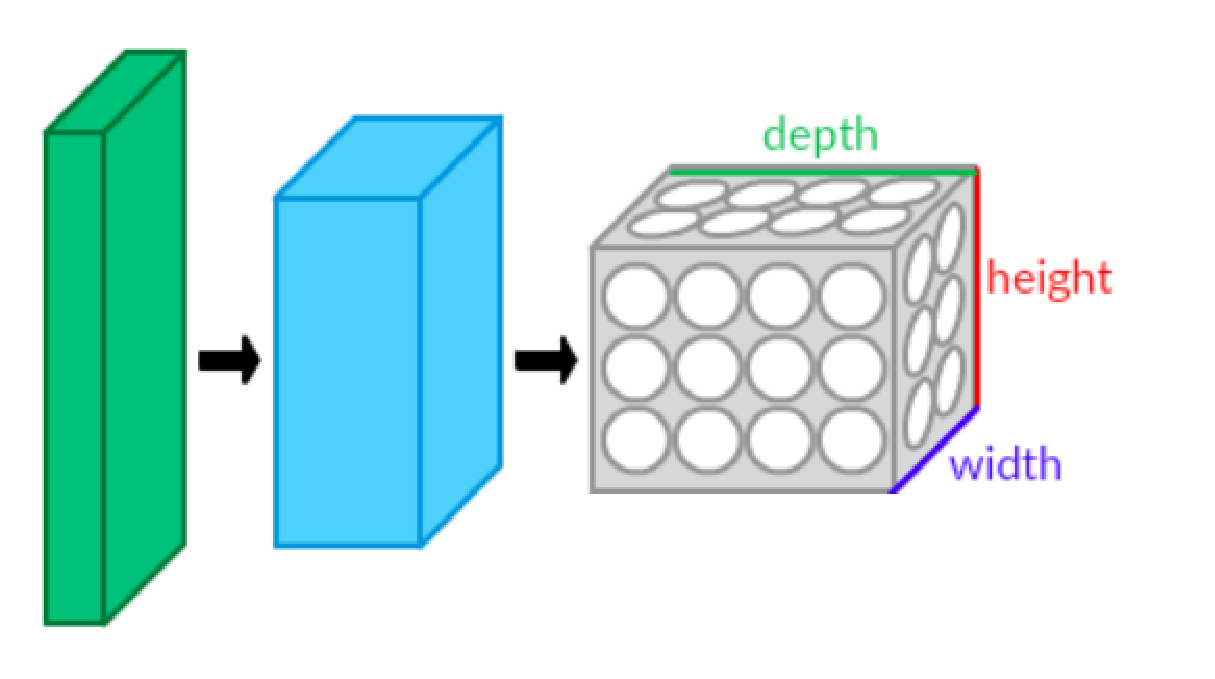
\includegraphics[scale=0.6]{imagens/Conv_layers.eps}
\caption{Para cada convolução, criamos uma nova imagem que possui uma
  nova largura (\textit{width} em inglês), altura (\textit{height} em
  inglês) e profundidade (\textit{depth} em inglês)}
\label{fig:convolution_kernel}
\end{figure}

Uma rede convolucional será basicamente uma rede neural de
profundidade. Ao invés de empilharmos camadas de multiplicação de
matrizes, estamos empilhando convoluções. Portanto no começo teremos
uma imagem grande que possui apenas os valores de pixel como
informação. Assim aplicamos convoluções que irão ``espremer'' as
dimensões espaciais e aumentar a profundidade. No final é possivel
conectar o classificador e ainda lidar apenas com parâmetros que
mapeiam o conteúdo da imagem.\cite{Dumoulin2016}

\subsubsection{Stride}

Quando estamos realizando uma convolução, deslizamos uma janela com o
tamanho do \textit{Kernel} pela imagem, o \textit{stride} é o
parâmetro que diz quantos pixels de espaçamento teremos entre um
fragmento da imagem e outro. Por exemplo um \textit{stride} de 1
significa que a imagem de saída pode ter a mesma largura e altura que
a imagem de entrada. Um valor de 2 significa que a imagem de saída
pode ter metade do tamanho.

\subsubsection{Padding}

O parâmetro de \textit{padding} é o que se faz nas bordas das imagens
de saída. Uma possibilidade é não deslizar o \textit{Kernel} até as
bordas da imagem, isso é chamado de {\bf \emph{valid padding}}. Outra
possibilidade é deslizar o seu \textit{Kernel} até as bordas da imagem
e completar com 0, essa técnica é chamada de {\bf \emph{same
    padding}}.

\begin{figure}[H]
\centering
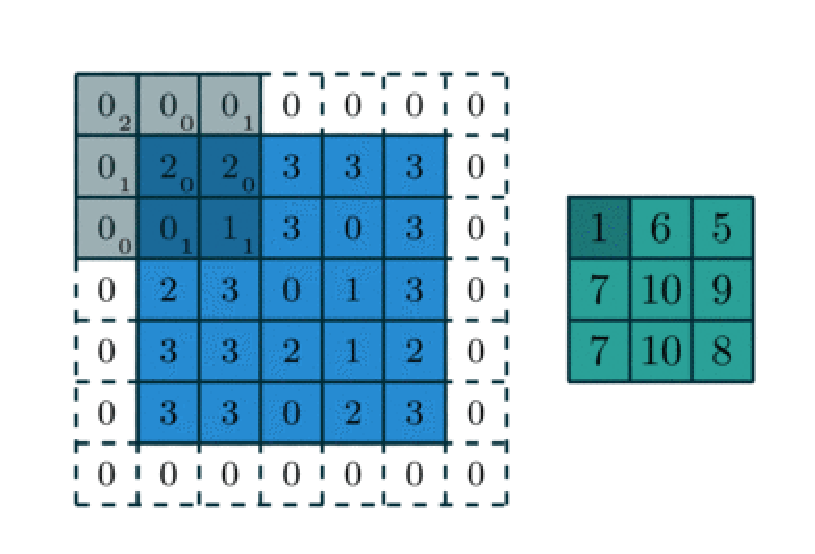
\includegraphics[scale=0.6]{imagens/conv_kernel_pad_stride.eps}
\caption{No exemplo temos uma imagem representada por uma matriz 5x5 e
  está sendo aplicado um \textit{kernel} de tamanho 3x3, com o
  \textit{stride} igual a 2 e um \textit{same padding}, completando as
  bordas com 0. Isso gera uma nova imagem 3x3 por consequência dos
  parâmetros escolhidos.}
\label{fig:conv_kernel_pad_stride}
\end{figure}

\subsection{Pooling}

Reduzir as dimensões espaciais da rede neural é primordial para
uma arquitetura eficaz do modelo. No entanto utilizar uma convolução
com \textit{stride} igual a 2 para essa tarefa é uma forma agressiva e
arriscada para isso, pois é possível perder bastante informação no
processo. Ao invés disso, iremos realizar convoluções com
\textit{stride} igual a 1, sem perder nenhuma informação da imagem
original. Após a camada convolucional iremos adicionar uma camada de
\textit{pooling} que irá receber todas as convoluções e combiná-las de
alguma forma\cite{Dumoulin2016}.

\subsubsection{Max pooling}

Para cada ponto nos mapas de características essa operação
olha para uma pequena vizinhança ao redor deste ponto. Com esses
valores em mãos é possível calcular o valor máximo dessa vizinhança.

Esta técnica geralmente leva a modelos mais eficazes. Porém a
computação das convoluções com \textit{stride} menor pode se tornar mais
lenta. Além disso, agora será necessário trabalhar com mais parâmetros
para a rede neural, o tamanho de região de \textit{pooling} e o
parâmetro de \textit{stride} para o \textit{pooling}.

\subsection{Camada completamente conectada}

De acordo com Krizhevsky\cite{Krizhevsky}, uma camada completamente
conectada tem conexões com todas as ativações das camadas anteriores,
assim como em redes neurais comuns. Suas ativações podem ser
calculadas através de uma multiplicação de matrizes seguida da adição
do fator \textit{bias}.